\documentclass[11pt]{article}
\usepackage[utf8]{inputenc}	% Para caracteres en español
\usepackage{amsmath,amsthm,amsfonts,amssymb,amscd}
\usepackage{multirow,booktabs}
\usepackage[table]{xcolor}
\usepackage{fullpage}
\usepackage{lastpage}
\usepackage{enumitem}
\usepackage{fancyhdr}
\usepackage{mathrsfs}
\usepackage{wrapfig}
\usepackage{setspace}
\usepackage{calc}
\usepackage{multicol}
\usepackage{cancel}
\usepackage[retainorgcmds]{IEEEtrantools}
\usepackage[margin=1cm]{geometry}
\usepackage{amsmath}
\newlength{\tabcont}
\setlength{\parindent}{0.0in}
\setlength{\parskip}{0.05in}
\usepackage{empheq}
\usepackage{framed}
\usepackage[most]{tcolorbox}
\usepackage{xcolor}
\usepackage{graphicx}
\usepackage{listings}
% -- Basic formatting
\usepackage[utf8]{inputenc}
\usepackage[english]{babel}
\usepackage{times}
\usepackage{caption}
\usepackage{subcaption}
\usepackage{placeins}
\setlength{\parindent}{0pt}
\usepackage{indentfirst}% -- Defining colors:
\usepackage[dvipsnames]{xcolor}
\definecolor{codegreen}{rgb}{0,0.6,0}
\definecolor{codegray}{rgb}{0.5,0.5,0.5}
\definecolor{codepurple}{rgb}{0.58,0,0.82}
\definecolor{backcolour}{rgb}{0.95,0.95,0.92}% Definig a custom style:
\lstdefinestyle{mystyle}{
    backgroundcolor=\color{backcolour},   
    commentstyle=\color{codepurple},
    keywordstyle=\color{NavyBlue},
    numberstyle=\tiny\color{codegray},
    stringstyle=\color{codepurple},
    basicstyle=\ttfamily\footnotesize\bfseries,
    breakatwhitespace=false,         
    breaklines=true,                 
    captionpos=t,                    
    keepspaces=true,                 
    numbers=left,                    
    numbersep=5pt,                  
    showspaces=false,                
    showstringspaces=false,
    showtabs=false,                  
    tabsize=2
}% -- Setting up the custom style:
\lstset{style=mystyle}
\lstset{
  style=mystyle,
  framexleftmargin=3.5mm,
  rulesepcolor=\color{black},
  linewidth=0.6\linewidth,
  xleftmargin=12pt,
  aboveskip=12pt,
  belowskip=12pt
}
\colorlet{shadecolor}{orange!15}
\parindent 0in
\parskip 1pt
\geometry{margin=1in, headsep=0.25in}
\theoremstyle{definition}
\newtheorem{defn}{Definition}
\newtheorem{reg}{Rule}
\newtheorem{exer}{Exercise}
\newtheorem{note}{Note}
\graphicspath{ {./images/} }
\linespread{0.75}
\begin{document}
\setcounter{section}{0}
\title{MIE223 Lecture Notes}

\thispagestyle{empty}

\begin{center}
{\LARGE \bf Advanced NLP Text Processing}\\
{\large MIE223}\\
Winter 2025
\end{center}
\section{Advanced NLP Text Processing}
\subsection{NLP Text Processing Pipeline}
\begin{itemize}
  \item Document → Sections and Paragraphs
  \item Paragraphs → Sentences (sentence segmentation / extraction)
  \item Sentences → Tokens
  \item Tokens → Lemmas or Morphological Variants / Stems
  \item Tokens → Part-of-speech (POS) Tags
  \item Tokens, POS Tags → Phrase Chunks (Named entities and Keyphrases)
  \item Tokens, POS Tags → Parse Trees
  \item Augment above with coreference, entailment, sentiment, ...
\end{itemize}

nltk covers POS tagging,
phrase chunking
Stanford NLP toolkit
provides parsing,
coreference, NER.
\section{Part-of-Speech Tagging}

\subsection{Parts of Speech}
A simple but useful form of
linguistic analysis

\begin{itemize}
  \item Perhaps starting with Aristotle in the West (384–322 BCE), there
  was the idea of having parts of speech
  \begin{itemize}
    \item a.k.a lexical categories, word classes, “tags”, POS
  \end{itemize}
  \item It comes from Dionysius Thrax of Alexandria (c. 100 BCE) the
  idea that is still with us that there are 8 parts of speech
  \begin{itemize}
    \item The ones we teach today
    \begin{itemize}
      \item School grammar: noun, verb, adjective, adverb, preposition,
      conjunction, pronoun, interjection
    \end{itemize}
  \end{itemize}
\end{itemize}

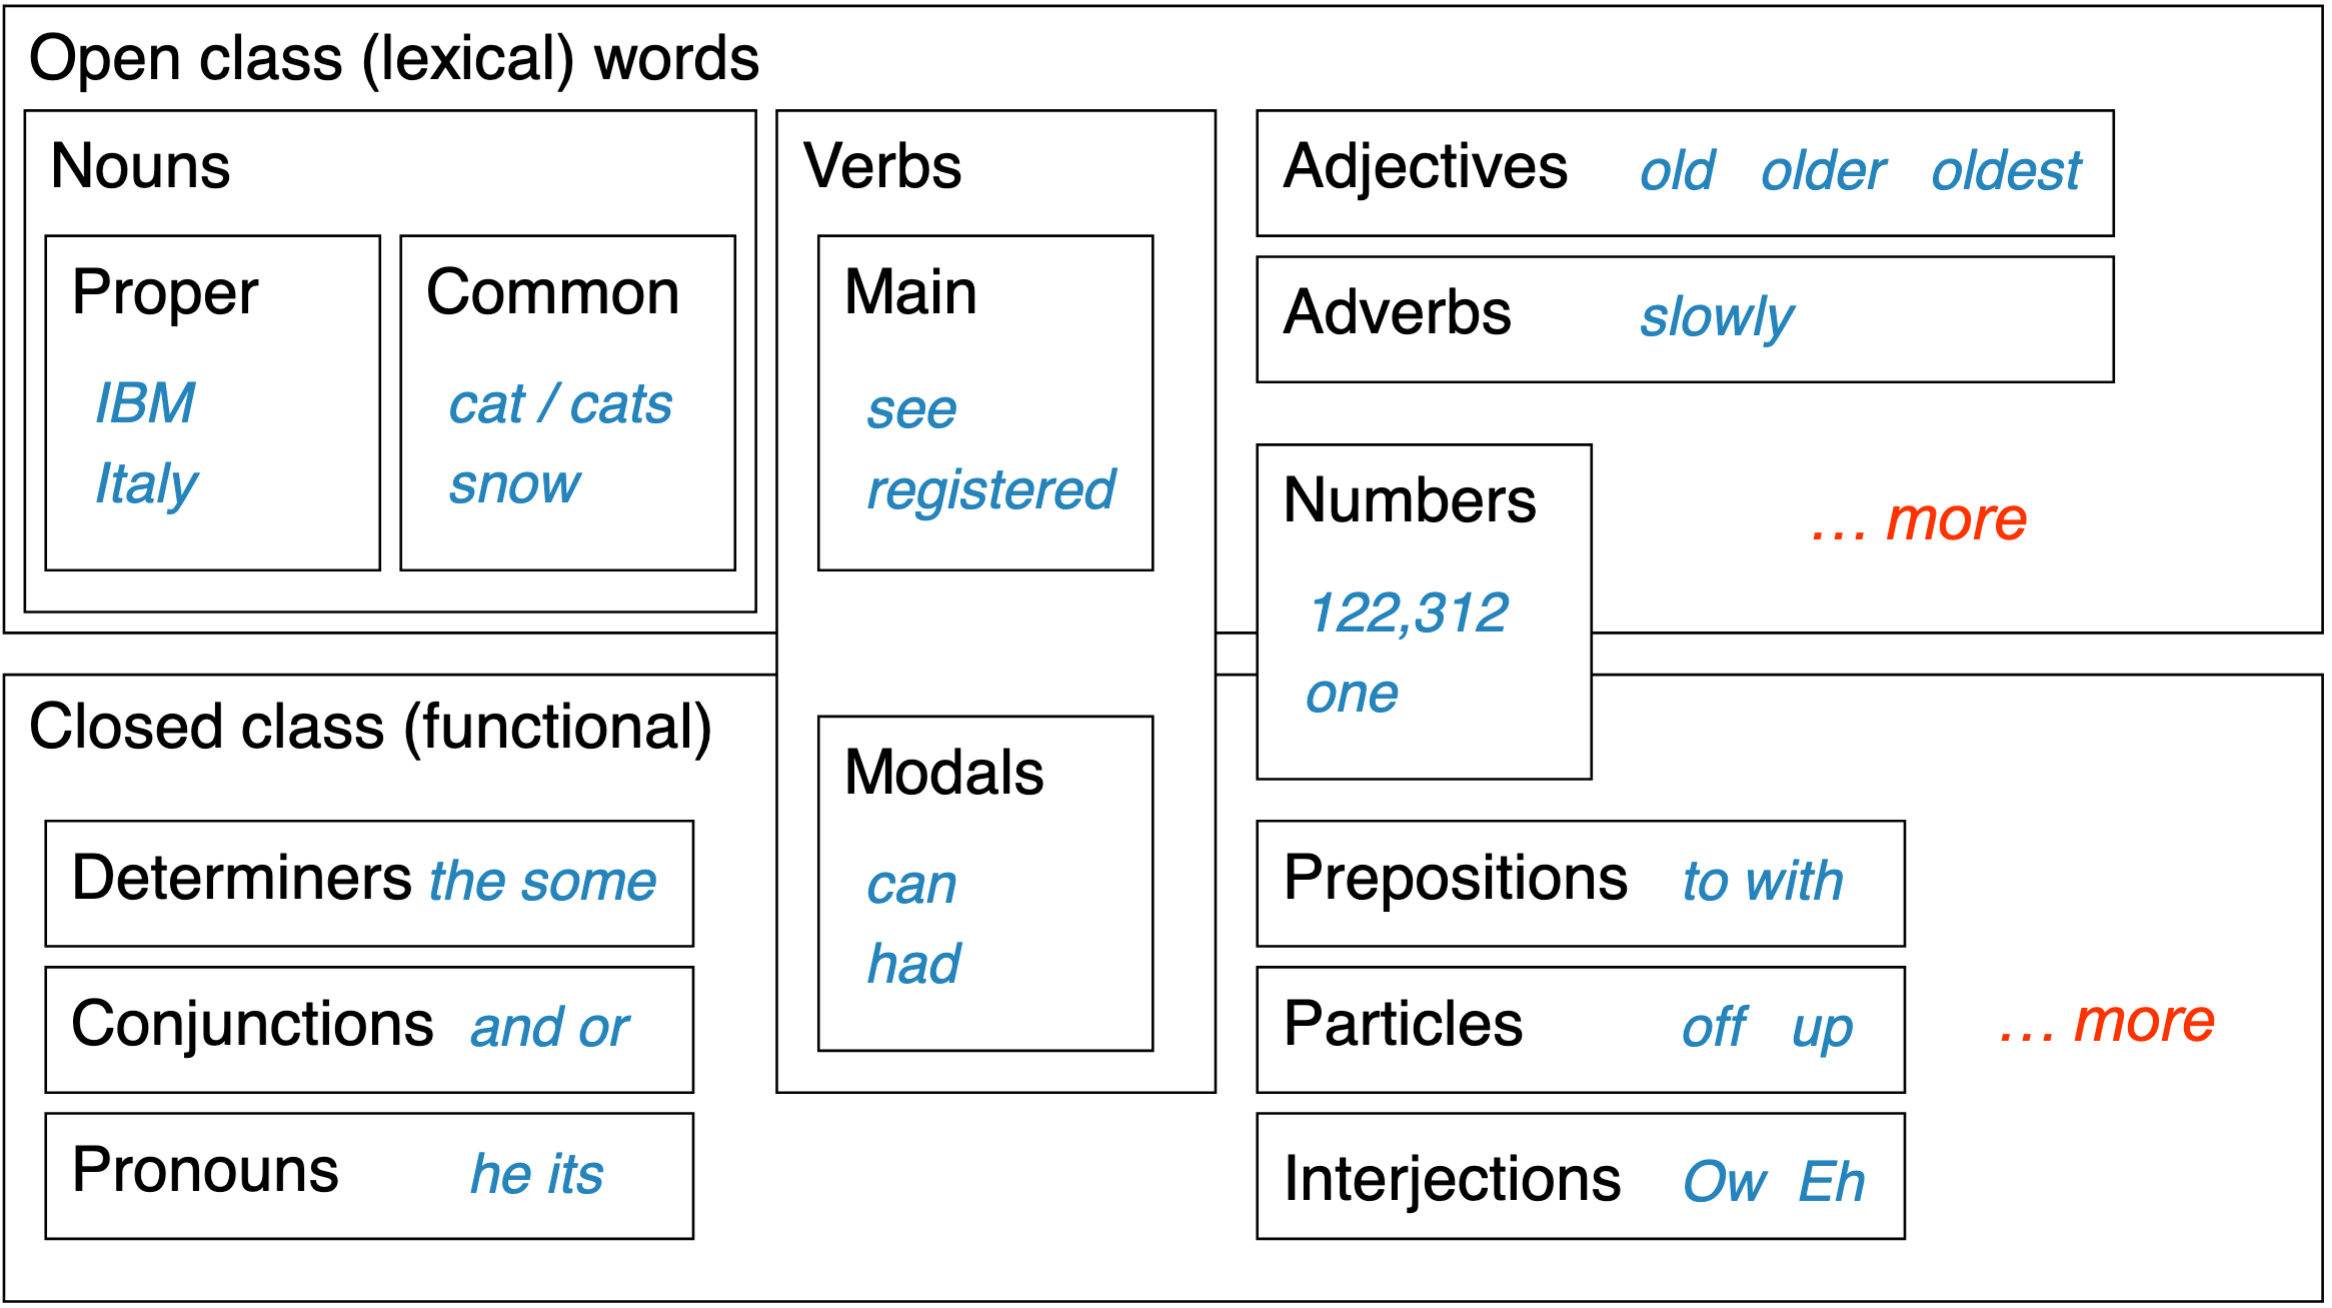
\includegraphics[width=\textwidth/2]{1.png}

\begin{verbatim}
  there are open classes and closed classes for words. 
  Open classes are nouns, verbs, adjectives, and adverbs.
  Closed classes are determiners, pronouns, prepositions, 
  and conjunctions.
\end{verbatim}

\subsection{Open vs. Closed classes}
Open vs. Closed classes

\begin{itemize}
  \item Closed:
  \begin{itemize}
    \item determiners: a, an, the
    \item pronouns: she, he, I
    \item prepositions: on, under, over, near, by, ...
    \item Why “closed”?
  \end{itemize}
  \item Open:
  \begin{itemize}
    \item Nouns, Verbs, Adjectives, Adverbs.
  \end{itemize}
\end{itemize}

\subsection{POS Tagging}
\begin{itemize}
  \item Words often have more than one POS: back
  \begin{itemize}
    \item The back door = JJ
    \item On my back = NN
    \item Win the voters back = RB
    \item Promised to back the bill = VB
  \end{itemize}
  \item The POS tagging problem is to determine the POS tag for a
  particular instance of a word.
\end{itemize}
\begin{itemize}
  \item Input: Plays well with others
  \item Ambiguity: NNS/VBZ UH/JJ/NN/RB IN NNS
  \item Output: Plays/VBZ well/RB with/IN others/NNS
  \item Uses:
  \begin{itemize}
    \item Text-to-speech (how do we pronounce “lead”, “record”, “wind”?)
    \item Can write regexps like (Det) Adj* N+ over the output for phrases, etc.
  \end{itemize}
\end{itemize}

\subsection{How difficult is POS tagging?}
\begin{itemize}
  \item About 11\% of the word types in the Brown corpus are
  ambiguous with regard to part of speech
  \item But they tend to be very common words. E.g., that
  \begin{itemize}
    \item I know that he is honest = IN
    \item Yes, that play was nice = DT
    \item You can’t go that far = RB
  \end{itemize}
  \item 40\% of the word tokens are ambiguous
\end{itemize}

\begin{verbatim}
  no POS tagging tested on exams.
\end{verbatim}

\section{Phrase Chunking and
Special Noun Phrases}

\subsection{Phrase Chunking}
Find all non-recursive noun phrases (NPs) and verb
phrases (VPs) in a sentence.

\begin{note}
  A phrase should not contain a subphrase of the same type.
  i.e. "New York Times" is a NP, but "New York" is not.
\end{note}

\begin{itemize}
  \item [] [NP I] [VP ate] [NP the spaghetti] [PP with] [NP meatballs].
  \item [] [NP He] [VP reckons] [NP the current account deficit] [VP will
  narrow] [PP to] [NP only \# 1.8 billion] [PP in] [NP September]
\end{itemize}

\subsection{Named Entity Recognition (NER)}
A special class of Proper Noun Phrases
\begin{itemize}
  \item People: Scott Sanner, President Obama, Madonna
  \item Places: New York, Madison Square Garden, Millenium Park
  \item Organizations: New York Times, University of Toronto
\end{itemize}

\subsection{Keyphrases}
\begin{itemize}
  \item Useful noun phrases, but not necessarily Proper Nouns, e.g.,
  \begin{itemize}
    \item “machine learning”
    \item “support vector machines”
    \item “genetically modified organisms”
  \end{itemize}
  \item A subset of frequent noun phrases (harder to extract than NEs)
  \begin{itemize}
    \item This paper has the best method I’ve found so far:
    “Automatic Recognition of Multi-Word Terms: the C-value/NC-value Method
    Katerina Frantziy, Sophia Ananiadouy, Hideki Mima” IJODL 2000.
    http://personalpages.manchester.ac.uk/staff/sophia.ananiadou/ijodl2000.pdf
  \end{itemize}
\end{itemize}

\section{Statistical Natural
Language Parsing}
Parsing: Two views of
syntactic structure

\subsection{Why parsing?}
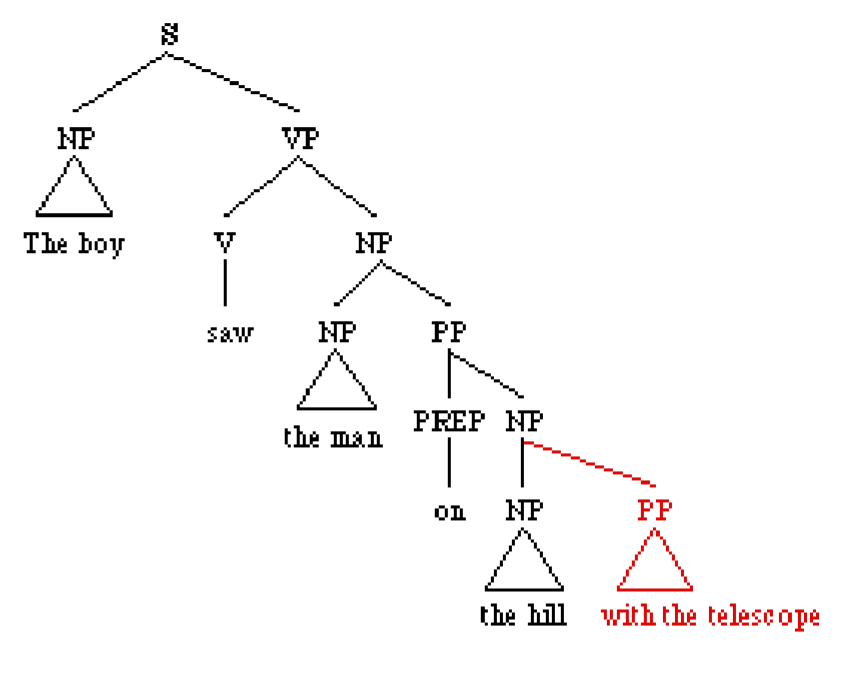
\includegraphics[width = \textwidth/2]{2.png}
\begin{itemize}
  \item “The boy saw the man on the hill with
  the telescope.”
  \begin{itemize}
    \item Who had the telescope?
  \end{itemize}
  \item Depends on whether you attach “with the telescope” to “I” or
  “man on the hill”
  \item How do you determine attachments? Parsing.
  \begin{itemize}
    \item Some sentences are inherently ambiguous: attachment ambiguity
  \end{itemize}
\end{itemize}

\subsection{Grammars for Parse Tree Production}
\begin{itemize}
  \item Parent → Child1 Child2 | Child3 Child4 ... | .
  \item S → NP VP | ...
  \item NP → ... NN* ...
  \item VP → ... VB* ...
  \item ADJP → ... JJ* ...
  \item ADVP → ... RB* ...
\end{itemize}

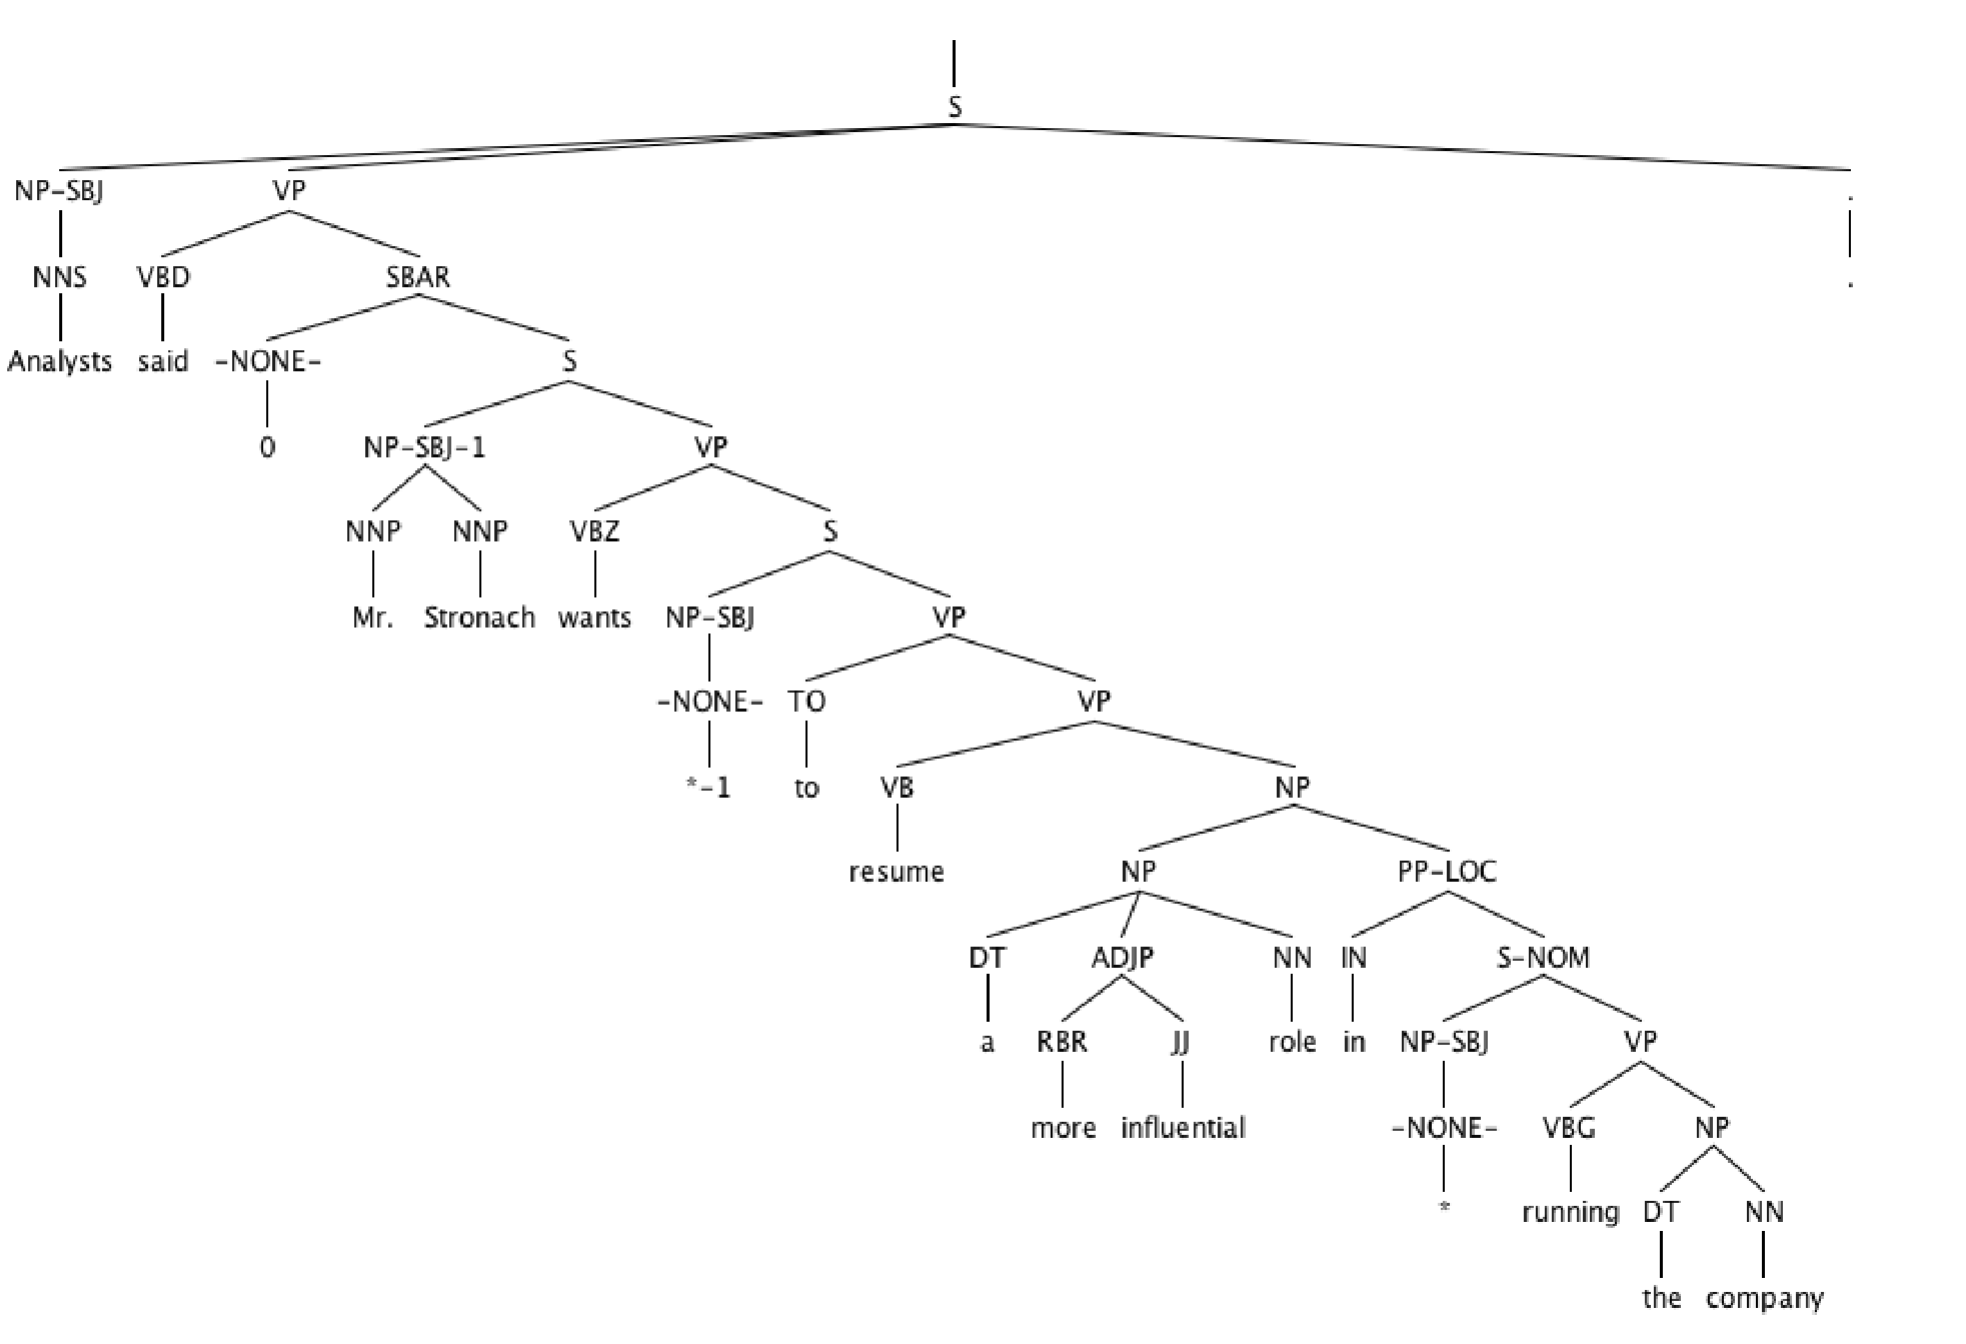
\includegraphics[width=\textwidth]{3.png}

\section{Semantic
Language Analysis}
Coreference and
entailment

\subsection{Coreference}
\begin{itemize}
  \item Discourse (multiple sentences) use coreferring phrases.
  \item Example:
  \begin{itemize}
    \item “John saw a beautiful Acura Integra in the dealership.
    He showed it to Bob.
    He bought it.”
  \end{itemize}
  \item What do “He” and “it” refer to in the 2nd sentence?
\end{itemize}

\subsection{Coreference Resolution}
\begin{itemize}
  \item “John saw a beautiful Acura Integra in the dealership.
  He1 showed it1 to Bob.
  He2 bought it2.”
  \item Important in processing reviews: “I liked it!”
\end{itemize}
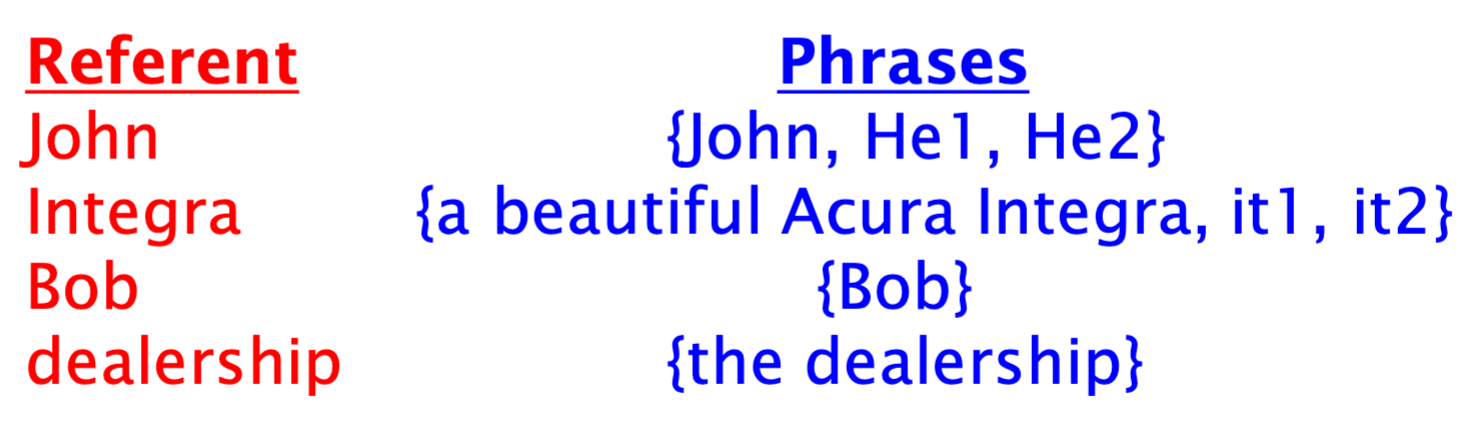
\includegraphics[width=\textwidth/2]{4.png}

\subsection{Entailment}
\begin{itemize}
  \item Question: When did the Berlin wall open?
  \item Text contains: The Berlin wall fell on November 9, 1989.
  \item Simple entailment? Does “fall” → “open”?
  \begin{itemize}
    \item A wall falling is a wall opening
    \item A person falling is not a person opening
  \end{itemize}
  \item Entailment can be highly contextual. But WordNet (in nltk)
  contains basic entailments, e.g., “snoring” → “sleeping”.
\end{itemize}
\end{document}